\documentclass{standalone}
\usepackage{tikz}
\usetikzlibrary{shapes.geometric}
\usepackage{ifthen}

\begin{document}

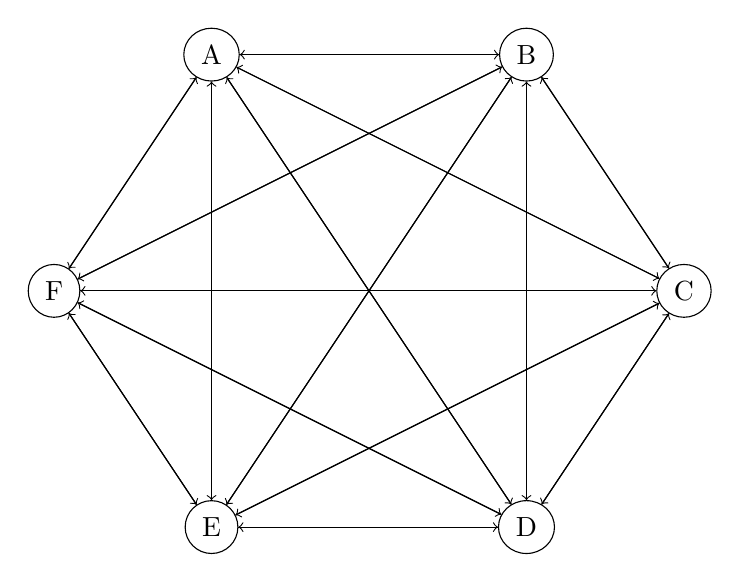
\begin{tikzpicture}
    \node[shape=ellipse,draw=black] (A) at (-2,5) {A};
    \node[shape=ellipse,draw=black] (B) at (2,5) {B};
    \node[shape=ellipse,draw=black] (C) at (4,2) {C};
    \node[shape=ellipse,draw=black] (D) at (2,-1) {D};
    \node[shape=ellipse,draw=black] (E) at (-2,-1) {E};
    \node[shape=ellipse,draw=black] (F) at (-4,2) {F};

    \foreach \i in {A,B,C,D,E,F} {
        \foreach \j in {A,B,C,D,E,F} {
            \ifthenelse{\equal{\i}{\j}}{}{\path [->] (\i) edge (\j);}
        }
    }
\end{tikzpicture}

\end{document}